\documentclass[8pt,aspectratio=169]{beamer}
\usetheme{Madrid}
\usepackage{graphicx}
\usepackage{booktabs}
\usepackage{adjustbox}
\usepackage{multicol}
\usepackage{amsmath}
\usepackage{amssymb}
\usepackage{tikz}
\usepackage{hyperref}
\usepackage{algorithm}
\usepackage{algorithmic}
\usepackage{colortbl}
\usepackage{pgfplots}
\pgfplotsset{compat=1.18}

% TikZ libraries for comics, diagrams, stakeholder maps
\usetikzlibrary{arrows.meta,positioning,shapes.callouts,shapes.geometric,decorations.pathreplacing}

% Color definitions
\definecolor{mlblue}{RGB}{0,102,204}
\definecolor{mlpurple}{RGB}{51,51,178}
\definecolor{mllavender}{RGB}{173,173,224}
\definecolor{mllavender2}{RGB}{193,193,232}
\definecolor{mllavender3}{RGB}{204,204,235}
\definecolor{mllavender4}{RGB}{214,214,239}
\definecolor{mlorange}{RGB}{255, 127, 14}
\definecolor{mlgreen}{RGB}{44, 160, 44}
\definecolor{mlred}{RGB}{214, 39, 40}
\definecolor{mlgray}{RGB}{127, 127, 127}
\definecolor{lightgray}{RGB}{240, 240, 240}
\definecolor{midgray}{RGB}{180, 180, 180}

% NEW COLORS for mini-lecture
\definecolor{dfteal}{RGB}{0,128,128}
\definecolor{dfred}{RGB}{180,30,30}

% Backward compatibility
\colorlet{MLPurple}{mlpurple}
\colorlet{MLBlue}{mlblue}
\colorlet{MLOrange}{mlorange}
\colorlet{MLGreen}{mlgreen}
\colorlet{MLRed}{mlred}
\colorlet{MLLavender}{mllavender}
\colorlet{MLGray}{mlgray}

% Theme colors (exact Madrid settings)
\setbeamercolor{palette primary}{bg=mllavender3,fg=mlpurple}
\setbeamercolor{palette secondary}{bg=mllavender2,fg=mlpurple}
\setbeamercolor{palette tertiary}{bg=mllavender,fg=white}
\setbeamercolor{palette quaternary}{bg=mlpurple,fg=white}
\setbeamercolor{structure}{fg=mlpurple}
\setbeamercolor{section in toc}{fg=mlpurple}
\setbeamercolor{subsection in toc}{fg=mlblue}
\setbeamercolor{title}{fg=mlpurple}
\setbeamercolor{frametitle}{fg=mlpurple,bg=mllavender3}
\setbeamercolor{block title}{bg=mllavender2,fg=mlpurple}
\setbeamercolor{block body}{bg=mllavender4,fg=black}
\setbeamertemplate{navigation symbols}{}
\setbeamertemplate{itemize items}[circle]
\setbeamertemplate{enumerate items}[default]
\setbeamersize{text margin left=5mm,text margin right=5mm}

% Footer
\setbeamertemplate{footline}{
  \leavevmode%
  \hbox{%
    \begin{beamercolorbox}[wd=.333333\paperwidth,ht=2.25ex,dp=1ex,center]{author in head/foot}%
      \usebeamerfont{author in head/foot}Methods and Algorithms
    \end{beamercolorbox}%
    \begin{beamercolorbox}[wd=.333333\paperwidth,ht=2.25ex,dp=1ex,center]{title in head/foot}%
      \usebeamerfont{title in head/foot}MSc Data Science
    \end{beamercolorbox}%
    \begin{beamercolorbox}[wd=.333333\paperwidth,ht=2.25ex,dp=1ex,right]{date in head/foot}%
      \usebeamerfont{date in head/foot}\insertframenumber{} / \inserttotalframenumber\hspace*{2ex}
    \end{beamercolorbox}}%
  \vskip0pt%
}

\newcommand{\bottomnote}[1]{%
\vfill
\vspace{-2mm}
\textcolor{mllavender2}{\rule{\textwidth}{0.4pt}}
\vspace{1mm}
\footnotesize
\textbf{#1}
}

\newenvironment{compactlist}{%
  \begin{itemize}%
    \setlength{\itemsep}{2pt}%
    \setlength{\parskip}{0pt}%
    \setlength{\parsep}{0pt}%
}{%
  \end{itemize}%
}

\newcommand{\highlight}[1]{\textcolor{mlorange}{\textbf{#1}}}
\newcommand{\mathbold}[1]{\boldsymbol{#1}}

\title[Linear Regression -- Full Lecture]{Linear Regression}
\subtitle{Full Technical Lecture}
\author{Methods \& Algorithms}
\date{MSc Data Science -- Spring 2026}

\begin{document}

%% ================================================================
%% ZONE 1: INTRODUCTION (frames 1-5, NO Greek, NO formulas)
%% ================================================================

\section{Introduction}

%% FRAME 1: Title Page
\begin{frame}[plain]
\titlepage
\end{frame}

%% FRAME 2: Opening XKCD
\begin{frame}[t]{Can You Really Just Draw a Line Through Anything?}
\begin{center}
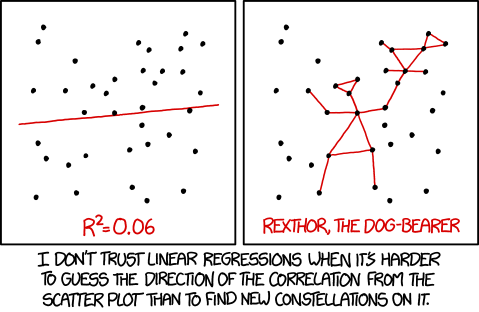
\includegraphics[width=0.55\textwidth]{images/1725_linear_regression.png}
\end{center}

\vspace{2mm}
\begin{center}
\small\textit{``I found a strong correlation between the number of people who\\drowned in swimming pools and the number of Nicolas Cage films.''}
\end{center}

\bottomnote{XKCD \#1725 by Randall Munroe (CC BY-NC 2.5)}
\end{frame}

%% FRAME 3: Problem Framing (SCQ)
\begin{frame}[t]{Why Do Banks Struggle to Value Properties Consistently?}
\begin{columns}[T]
\column{0.55\textwidth}
\small
\textbf{Situation}
\begin{compactlist}
\item A bank receives 500 mortgage applications per week
\item Each property has size, location, age, condition
\end{compactlist}

\vspace{2mm}
\textbf{Complication}
\begin{compactlist}
\item Human appraisers disagree by 10--20\%
\item Inconsistent valuations create risk
\end{compactlist}

\vspace{2mm}
\textbf{Question}
\begin{block}{}
\scriptsize Can we learn a systematic rule from past transactions that predicts price from features -- and quantifies uncertainty?
\end{block}

\column{0.42\textwidth}
\vspace{2mm}
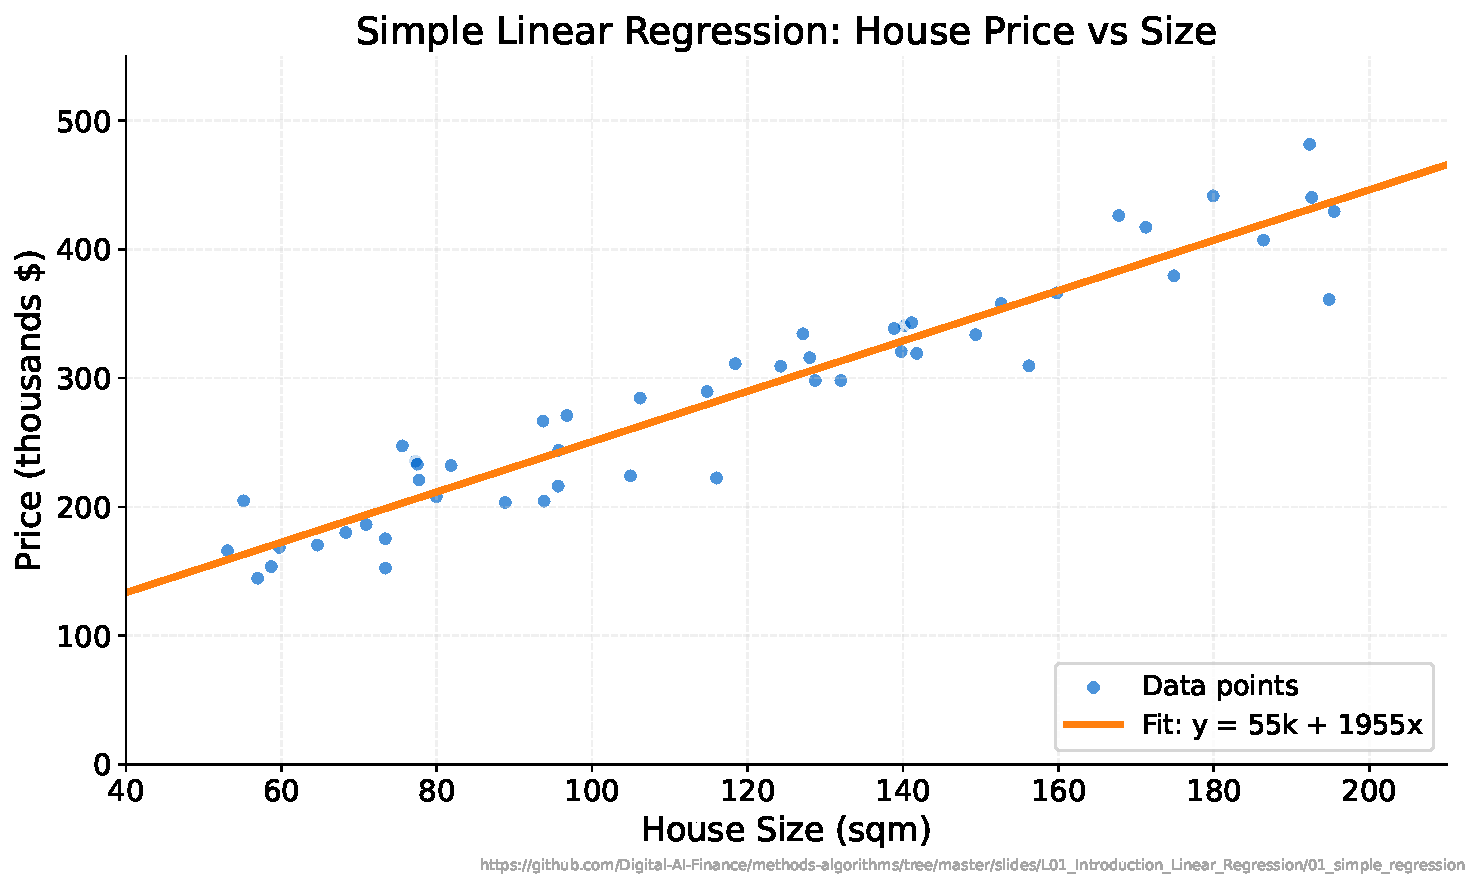
\includegraphics[width=\textwidth]{01_simple_regression/chart.pdf}
\end{columns}

\bottomnote{Linear regression turns this question into a mathematical optimization problem with a unique, closed-form solution}
\end{frame}

%% FRAME 4: Learning Objectives
\begin{frame}[t]{What Will You Be Able to Do After This Lecture?}
\small
\begin{enumerate}
\setlength{\itemsep}{8pt}
\item \highlight{Derive} the OLS estimator from the loss function using matrix calculus, and explain each step of the derivation
\item \highlight{Analyze} residual plots, multicollinearity diagnostics, and learning curves to detect model violations
\item \highlight{Evaluate} when Ridge, Lasso, or Elastic Net regularization is appropriate for a given dataset
\item \highlight{Compare} linear regression with gradient-descent-based optimization and select the right approach for the problem scale
\end{enumerate}

\bottomnote{All four objectives target Bloom's levels 4--5 (Analyze, Evaluate, Compare)}
\end{frame}

%% FRAME 5: Roadmap
\begin{frame}[t]{Roadmap: From Scatter Plot to Production Model}
\begin{center}
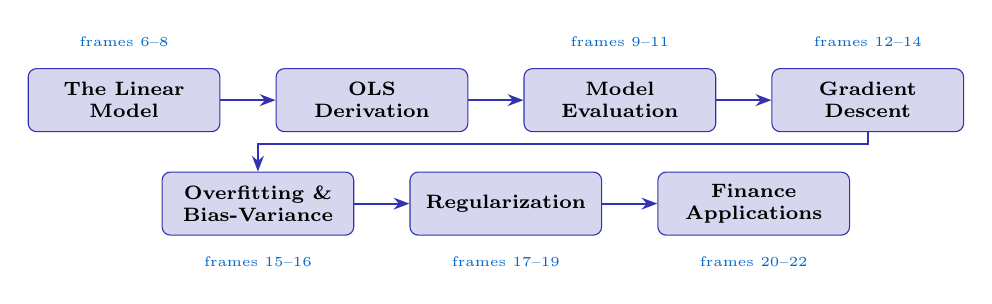
\begin{tikzpicture}[
  node distance=0.3cm and 0.7cm,
  box/.style={rectangle, rounded corners=3pt, draw=mlpurple, fill=mllavender4, text width=2.2cm, minimum height=0.8cm, align=center, font=\scriptsize\bfseries},
  arr/.style={-{Stealth[length=2mm]}, thick, mlpurple}
]
\node[box] (m1) {The Linear\\Model};
\node[box, right=of m1] (m2) {OLS\\Derivation};
\node[box, right=of m2] (m3) {Model\\Evaluation};
\node[box, right=of m3] (m4) {Gradient\\Descent};
\node[box, below=0.5cm of m1, xshift=1.7cm] (m5) {Overfitting \&\\Bias-Variance};
\node[box, right=of m5] (m6) {Regularization};
\node[box, right=of m6] (m7) {Finance\\Applications};

\draw[arr] (m1) -- (m2);
\draw[arr] (m2) -- (m3);
\draw[arr] (m3) -- (m4);
\draw[arr] (m4.south) -- ++(0,-0.15) -| (m5.north);
\draw[arr] (m5) -- (m6);
\draw[arr] (m6) -- (m7);

% Section labels
\node[font=\tiny, mlblue, above=0.15cm of m1] {frames 6--8};
\node[font=\tiny, mlblue, above=0.15cm of m3] {frames 9--11};
\node[font=\tiny, mlblue, above=0.15cm of m4] {frames 12--14};
\node[font=\tiny, mlblue, below=0.15cm of m5] {frames 15--16};
\node[font=\tiny, mlblue, below=0.15cm of m6] {frames 17--19};
\node[font=\tiny, mlblue, below=0.15cm of m7] {frames 20--22};
\end{tikzpicture}
\end{center}

\vspace{4mm}
\begin{center}
\small Each block builds on the previous one. By the end, you will have a complete toolkit for building, evaluating, and regularizing linear models.
\end{center}

\bottomnote{We follow the PMSP framework: Problem -- Method -- Solution -- Practice}
\end{frame}

%% ================================================================
%% ZONE 2: CORE (frames 6-22, formulas OK)
%% ================================================================

\section{The Linear Model}

%% FRAME 6: The Linear Model
\begin{frame}[t]{How Do We Write the Linear Model in Matrix Form?}
\begin{columns}[T]
\column{0.52\textwidth}
\small
\textbf{Scalar form} (single observation):
\[\hat{y}_i = \beta_0 + \beta_1 x_{i1} + \beta_2 x_{i2} + \cdots + \beta_p x_{ip}\]

\textbf{Matrix form} (all $n$ observations):
\[\hat{\mathbf{y}} = X\boldsymbol{\beta}\]

\begin{compactlist}
\item $X$ is the $n \times (p{+}1)$ \highlight{design matrix} (column of 1s for intercept)
\item $\boldsymbol{\beta}$ is the $(p{+}1) \times 1$ coefficient vector
\item $\hat{\mathbf{y}}$ is the $n \times 1$ prediction vector
\end{compactlist}

\column{0.45\textwidth}
\vspace{2mm}
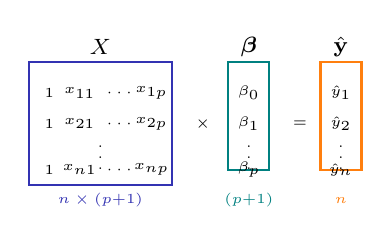
\begin{tikzpicture}[scale=0.65, font=\tiny]
% X matrix
\draw[mlpurple, thick] (0,0) rectangle (2.8,2.4);
\node at (1.4,2.7) {\footnotesize $X$};
\node at (0.4,1.8) {1};  \node at (1.0,1.8) {$x_{11}$}; \node at (1.8,1.8) {$\cdots$}; \node at (2.4,1.8) {$x_{1p}$};
\node at (0.4,1.2) {1};  \node at (1.0,1.2) {$x_{21}$}; \node at (1.8,1.2) {$\cdots$}; \node at (2.4,1.2) {$x_{2p}$};
\node at (1.4,0.7) {$\vdots$};
\node at (0.4,0.3) {1};  \node at (1.0,0.3) {$x_{n1}$}; \node at (1.8,0.3) {$\cdots$}; \node at (2.4,0.3) {$x_{np}$};
% beta vector
\node at (3.4,1.2) {$\times$};
\draw[dfteal, thick] (3.9,0.3) rectangle (4.7,2.4);
\node at (4.3,2.7) {\footnotesize $\boldsymbol{\beta}$};
\node at (4.3,1.8) {$\beta_0$};
\node at (4.3,1.2) {$\beta_1$};
\node at (4.3,0.7) {$\vdots$};
\node at (4.3,0.3) {$\beta_p$};
% equals y
\node at (5.3,1.2) {$=$};
\draw[mlorange, thick] (5.7,0.3) rectangle (6.5,2.4);
\node at (6.1,2.7) {\footnotesize $\hat{\mathbf{y}}$};
\node at (6.1,1.8) {$\hat{y}_1$};
\node at (6.1,1.2) {$\hat{y}_2$};
\node at (6.1,0.7) {$\vdots$};
\node at (6.1,0.3) {$\hat{y}_n$};
% Dimension labels
\node[mlpurple, font=\tiny] at (1.4,-0.3) {$n \times (p{+}1)$};
\node[dfteal, font=\tiny] at (4.3,-0.3) {$(p{+}1)$};
\node[mlorange, font=\tiny] at (6.1,-0.3) {$n$};
\end{tikzpicture}
\end{columns}

\bottomnote{The column of 1s in $X$ absorbs the intercept $\beta_0$ into the matrix product -- no special case needed}
\end{frame}

%% FRAME 7: OLS Derivation
\begin{frame}[t]{How Does OLS Find the Best Line?}
\small
\textbf{Step 1: Define the loss}
\vspace{-1mm}
\[L(\boldsymbol{\beta}) = \|\mathbf{y} - X\boldsymbol{\beta}\|^2 = (\mathbf{y} - X\boldsymbol{\beta})^T(\mathbf{y} - X\boldsymbol{\beta})\]

\textbf{Step 2: Expand}
\vspace{-1mm}
\[L = \mathbf{y}^T\mathbf{y} - 2\boldsymbol{\beta}^TX^T\mathbf{y} + \boldsymbol{\beta}^TX^TX\boldsymbol{\beta}\]

\textbf{Step 3: Differentiate and set to zero}
\vspace{-1mm}
\[\frac{\partial L}{\partial \boldsymbol{\beta}} = -2X^T\mathbf{y} + 2X^TX\boldsymbol{\beta} = \mathbf{0}\]

\textbf{Step 4: Solve the normal equations}
\vspace{-1mm}
\[X^TX\boldsymbol{\beta} = X^T\mathbf{y} \quad \Longrightarrow \quad \boxed{\hat{\boldsymbol{\beta}} = (X^TX)^{-1}X^T\mathbf{y}}\]

\bottomnote{The loss is convex (quadratic), so this unique solution is the global minimum. Requires $X^TX$ invertible (no perfect multicollinearity).}
\end{frame}

%% FRAME 8: OLS Worked Example
\begin{frame}[t]{Can We Compute OLS by Hand?}
\small
\textbf{Data}: 4 houses with size (100s sqft) $\to$ price (\$1000s)

\vspace{1mm}
\begin{columns}[T]
\column{0.45\textwidth}
\footnotesize
\begin{tabular}{ccc}
\toprule
$i$ & $x_i$ & $y_i$ \\
\midrule
1 & 1 & 2 \\
2 & 2 & 3 \\
3 & 3 & 5 \\
4 & 4 & 6 \\
\bottomrule
\end{tabular}

\vspace{3mm}
$X = \begin{pmatrix} 1 & 1 \\ 1 & 2 \\ 1 & 3 \\ 1 & 4 \end{pmatrix}, \quad \mathbf{y} = \begin{pmatrix} 2 \\ 3 \\ 5 \\ 6 \end{pmatrix}$

\column{0.52\textwidth}
\footnotesize
$X^TX = \begin{pmatrix} 4 & 10 \\ 10 & 30 \end{pmatrix}, \quad X^T\mathbf{y} = \begin{pmatrix} 16 \\ 49 \end{pmatrix}$

\vspace{2mm}
$(X^TX)^{-1} = \frac{1}{20}\begin{pmatrix} 30 & -10 \\ -10 & 4 \end{pmatrix}$

\vspace{2mm}
$\hat{\boldsymbol{\beta}} = \frac{1}{20}\begin{pmatrix} 30 & -10 \\ -10 & 4 \end{pmatrix}\begin{pmatrix} 16 \\ 49 \end{pmatrix} = \begin{pmatrix} -0.5 \\ 1.6 \end{pmatrix}$

\vspace{2mm}
\highlight{Result}: $\hat{y} = -0.5 + 1.6x$

$R^2 = 1 - \frac{1.40}{10} = 0.86$
\end{columns}

\bottomnote{Verify: $\hat{y}_1 = 1.1$ (residual $0.9$), $\hat{y}_2 = 2.7$ (residual $0.3$), $\hat{y}_3 = 4.3$ (residual $0.7$), $\hat{y}_4 = 5.9$ (residual $0.1$)}
\end{frame}

\section{Model Evaluation}

%% FRAME 9: Model Evaluation
\begin{frame}[t]{How Do We Know If the Model Is Any Good?}
\begin{columns}[T]
\column{0.55\textwidth}
\small
\textbf{$R^2$: Proportion of variance explained}
\[R^2 = 1 - \frac{\text{SS}_{\text{res}}}{\text{SS}_{\text{tot}}} = 1 - \frac{\sum(y_i - \hat{y}_i)^2}{\sum(y_i - \bar{y})^2}\]

\begin{compactlist}
\item $R^2 = 1$: perfect predictions
\item $R^2 = 0$: no better than predicting the mean
\item \highlight{Adjusted $R^2$} penalizes adding useless features:
\end{compactlist}

\vspace{1mm}
\[R^2_{\text{adj}} = 1 - \frac{(1-R^2)(n-1)}{n-p-1}\]

\begin{block}{Warning}
\scriptsize High $R^2$ does not mean correct model. Always inspect residuals.
\end{block}

\column{0.42\textwidth}
\vspace{2mm}

\includegraphics[width=\textwidth]{03_residual_plots/chart.pdf}
\end{columns}

\bottomnote{$R^2$ can only increase with more features -- adjusted $R^2$ guards against overfitting by penalizing model complexity}
\end{frame}

%% FRAME 10: Residual Analysis
\begin{frame}[t]{What Do Residual Patterns Tell Us?}
\small
\begin{columns}[T]
\column{0.48\textwidth}
\textbf{Good residuals} (random scatter):
\begin{compactlist}
\item No visible pattern around zero
\item Constant spread (homoscedasticity)
\item Approximately normal distribution
\end{compactlist}

\vspace{3mm}
\textbf{Bad residuals} (systematic patterns):
\begin{compactlist}
\item \highlight{Funnel shape}: heteroscedasticity -- variance changes with $\hat{y}$
\item \highlight{Curved pattern}: non-linearity -- need polynomial or transform
\item \highlight{Clusters}: missing categorical variable
\end{compactlist}

\column{0.48\textwidth}
\vspace{2mm}
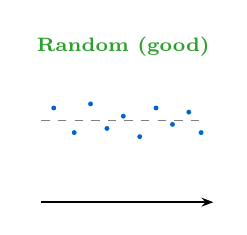
\begin{tikzpicture}[scale=0.52, font=\tiny]
% Good residuals
\node[font=\scriptsize\bfseries, mlgreen] at (2,3.8) {Random (good)};
\draw[-{Stealth[length=1.5mm]}, thick] (0,0) -- (4.2,0);
\draw[mlgray, dashed] (0,2) -- (4,2);
\fill[mlblue] (0.3,2.3) circle (0.06); \fill[mlblue] (0.8,1.7) circle (0.06);
\fill[mlblue] (1.2,2.4) circle (0.06); \fill[mlblue] (1.6,1.8) circle (0.06);
\fill[mlblue] (2.0,2.1) circle (0.06); \fill[mlblue] (2.4,1.6) circle (0.06);
\fill[mlblue] (2.8,2.3) circle (0.06); \fill[mlblue] (3.2,1.9) circle (0.06);
\fill[mlblue] (3.6,2.2) circle (0.06); \fill[mlblue] (3.9,1.7) circle (0.06);
\end{tikzpicture}

\vspace{3mm}
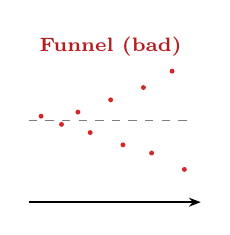
\begin{tikzpicture}[scale=0.52, font=\tiny]
% Bad residuals - funnel
\node[font=\scriptsize\bfseries, dfred] at (2,3.8) {Funnel (bad)};
\draw[-{Stealth[length=1.5mm]}, thick] (0,0) -- (4.2,0);
\draw[mlgray, dashed] (0,2) -- (4,2);
\fill[mlred] (0.3,2.1) circle (0.06); \fill[mlred] (0.8,1.9) circle (0.06);
\fill[mlred] (1.2,2.2) circle (0.06); \fill[mlred] (1.5,1.7) circle (0.06);
\fill[mlred] (2.0,2.5) circle (0.06); \fill[mlred] (2.3,1.4) circle (0.06);
\fill[mlred] (2.8,2.8) circle (0.06); \fill[mlred] (3.0,1.2) circle (0.06);
\fill[mlred] (3.5,3.2) circle (0.06); \fill[mlred] (3.8,0.8) circle (0.06);
\end{tikzpicture}
\end{columns}

\bottomnote{LINE assumptions: Linearity, Independence, Normality of residuals, Equal variance (homoscedasticity)}
\end{frame}

%% FRAME 11: Multiple Regression
\begin{frame}[t]{What Changes When We Add More Features?}
\begin{columns}[T]
\column{0.55\textwidth}
\small
\textbf{From 1D line to $p$-dimensional hyperplane}
\begin{compactlist}
\item With $p$ features, OLS fits a hyperplane in $(p{+}1)$-dimensional space
\item Each $\beta_j$ measures the effect of $x_j$ \emph{holding all other features constant} (ceteris paribus)
\item \highlight{Multicollinearity}: if features are correlated, coefficient estimates become unstable
\end{compactlist}

\vspace{2mm}
\begin{block}{Variance Inflation Factor}
\scriptsize $\text{VIF}_j = \frac{1}{1 - R^2_j}$ where $R^2_j$ is from regressing $x_j$ on all other features. VIF $> 10$ signals serious collinearity.
\end{block}

\column{0.42\textwidth}
\vspace{2mm}

\includegraphics[width=\textwidth]{02_multiple_regression_3d/chart.pdf}
\end{columns}

\bottomnote{In 3D the regression surface is a plane. In higher dimensions it is a hyperplane -- the math is identical.}
\end{frame}

\section{Optimization}

%% FRAME 12: Gradient Descent
\begin{frame}[t]{Why Not Always Use the Closed-Form Solution?}
\begin{columns}[T]
\column{0.55\textwidth}
\small
\textbf{OLS cost}: $O(np^2 + p^3)$ for matrix inversion

When $n$ or $p$ is very large, this becomes prohibitive.

\vspace{2mm}
\textbf{Gradient descent alternative}:
\[\boldsymbol{\beta}_{t+1} = \boldsymbol{\beta}_t - \alpha \nabla L(\boldsymbol{\beta}_t)\]

\begin{compactlist}
\item $\alpha$ is the \highlight{learning rate}
\item $\nabla L = -\frac{2}{n}X^T(\mathbf{y} - X\boldsymbol{\beta})$ (gradient of MSE)
\item Each step costs $O(np)$ -- scales linearly
\item Converges to the same solution as OLS
\end{compactlist}

\column{0.42\textwidth}
\vspace{2mm}

\includegraphics[width=\textwidth]{04_gradient_descent/chart.pdf}
\end{columns}

\bottomnote{OLS: exact but $O(p^3)$. Gradient descent: iterative but $O(np)$ per step. For $n > 10{,}000$ or $p > 1{,}000$, GD wins.}
\end{frame}

%% FRAME 13: Gradient Descent Variants
\begin{frame}[t]{Which Flavor of Gradient Descent Should You Use?}
\small
\begin{columns}[T]
\column{0.48\textwidth}
\textbf{Batch GD}
\begin{compactlist}
\item Uses \emph{all} $n$ samples per step
\item Smooth convergence, expensive per step
\item Best for small-to-medium data
\end{compactlist}

\vspace{3mm}
\textbf{Stochastic GD (SGD)}
\begin{compactlist}
\item Uses \emph{one} random sample per step
\item Noisy updates, very fast per step
\item Can escape local minima (non-convex)
\end{compactlist}

\column{0.48\textwidth}
\textbf{Mini-batch GD}
\begin{compactlist}
\item Uses a batch of $b$ samples (e.g., $b = 32$)
\item Best of both: stable yet fast
\item Standard choice in deep learning
\end{compactlist}

\vspace{3mm}
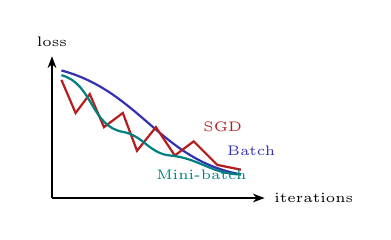
\begin{tikzpicture}[scale=0.6, font=\tiny]
\draw[-{Stealth[length=1.5mm]}] (0,0) -- (4.5,0) node[right] {iterations};
\draw[-{Stealth[length=1.5mm]}] (0,0) -- (0,3) node[above] {loss};
% Batch: smooth curve
\draw[mlpurple, thick] (0.2,2.7) to[out=-15,in=170] (4,0.5);
\node[mlpurple, right, font=\tiny] at (3.5,1.0) {Batch};
% SGD: noisy
\draw[dfred, thick] (0.2,2.5) -- (0.5,1.8) -- (0.8,2.2) -- (1.1,1.5) -- (1.5,1.8) -- (1.8,1.0) -- (2.2,1.5) -- (2.6,0.9) -- (3.0,1.2) -- (3.5,0.7) -- (4,0.6);
\node[dfred, right, font=\tiny] at (3.0,1.5) {SGD};
% Mini-batch: mild noise
\draw[dfteal, thick] (0.2,2.6) to[out=-15,in=170] (1.5,1.4) to[out=-10,in=175] (2.5,0.9) to[out=-5,in=180] (4,0.5);
\node[dfteal, right, font=\tiny] at (2.0,0.5) {Mini-batch};
\end{tikzpicture}
\end{columns}

\bottomnote{For linear regression (convex loss), all three converge to the same optimum. The choice is about computational cost.}
\end{frame}

%% FRAME 14: Learning Rate
\begin{frame}[t]{How Does the Learning Rate Affect Convergence?}
\begin{center}
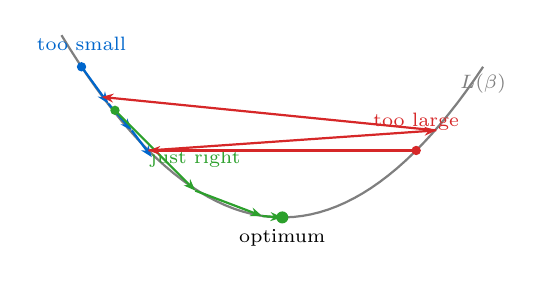
\begin{tikzpicture}[scale=0.85, font=\small]
% Loss surface (parabola)
\draw[mlgray, thick, domain=0.2:6.5, samples=50] plot (\x, {0.25*(\x-3.5)^2 + 0.5});

% Too small
\fill[mlblue] (0.5,2.75) circle (0.07);
\draw[-{Stealth[length=1.5mm]}, mlblue, thick] (0.5,2.75) -- (0.9,2.2);
\draw[-{Stealth[length=1.5mm]}, mlblue, thick] (0.9,2.2) -- (1.25,1.8);
\draw[-{Stealth[length=1.5mm]}, mlblue, thick] (1.25,1.8) -- (1.55,1.4);
\node[mlblue, font=\scriptsize, above] at (0.5,2.85) {too small};

% Just right
\fill[mlgreen] (1.0,2.1) circle (0.07);
\draw[-{Stealth[length=1.5mm]}, mlgreen, thick] (1.0,2.1) -- (2.2,0.9);
\draw[-{Stealth[length=1.5mm]}, mlgreen, thick] (2.2,0.9) -- (3.2,0.52);
\draw[-{Stealth[length=1.5mm]}, mlgreen, thick] (3.2,0.52) -- (3.5,0.5);
\fill[mlgreen] (3.5,0.5) circle (0.09);
\node[mlgreen, font=\scriptsize, above] at (2.2,1.1) {just right};

% Too large
\fill[mlred] (5.5,1.5) circle (0.07);
\draw[-{Stealth[length=1.5mm]}, mlred, thick] (5.5,1.5) -- (1.5,1.5);
\draw[-{Stealth[length=1.5mm]}, mlred, thick] (1.5,1.5) -- (5.8,1.8);
\draw[-{Stealth[length=1.5mm]}, mlred, thick] (5.8,1.8) -- (0.8,2.3);
\node[mlred, font=\scriptsize, above] at (5.5,1.65) {too large};

% Labels
\node[font=\scriptsize] at (3.5,0.2) {optimum};
\node[font=\scriptsize, mlgray] at (6.5,2.5) {$L(\beta)$};
\end{tikzpicture}
\end{center}

\begin{compactlist}
\item \textcolor{mlblue}{\textbf{Too small}}: converges but wastes computation -- may need thousands of steps
\item \textcolor{mlgreen}{\textbf{Just right}}: reaches the optimum in a few steps
\item \textcolor{mlred}{\textbf{Too large}}: overshoots and diverges -- the loss increases
\end{compactlist}

\bottomnote{In practice, use learning rate schedules or adaptive methods (Adam, RMSProp) that adjust $\alpha$ automatically}
\end{frame}

\section{Model Evaluation}

%% FRAME 15: Learning Curves
\begin{frame}[t]{How Do Training and Validation Error Behave?}
\begin{columns}[T]
\column{0.55\textwidth}
\small
\textbf{Learning curves} plot error vs.\ training set size:
\begin{compactlist}
\item \highlight{Training error} starts low, increases with more data (harder to memorize)
\item \highlight{Validation error} starts high, decreases with more data (better generalization)
\item The \highlight{gap} between them diagnoses the problem
\end{compactlist}

\vspace{2mm}
\begin{block}{Diagnostic Rules}
\scriptsize
\textbf{High bias}: both curves plateau high $\to$ model too simple\\
\textbf{High variance}: large gap $\to$ model too complex, need more data or regularization
\end{block}

\column{0.42\textwidth}
\vspace{2mm}

\includegraphics[width=\textwidth]{05_learning_curves/chart.pdf}
\end{columns}

\bottomnote{Learning curves are the single best diagnostic for deciding whether you need more data, more features, or regularization}
\end{frame}

%% FRAME 16: Overfitting & Bias-Variance
\begin{frame}[t]{What Is the Bias-Variance Tradeoff?}
\begin{columns}[T]
\column{0.55\textwidth}
\small
\textbf{Expected test error decomposes as}:
\[\text{MSE} = \text{Bias}^2 + \text{Variance} + \text{Irreducible Noise}\]

\begin{compactlist}
\item \highlight{Bias}: error from wrong assumptions (e.g., fitting a line to a curve)
\item \highlight{Variance}: sensitivity to training data fluctuations
\item As model complexity increases: bias decreases, variance increases
\item The optimum is where their sum is minimized
\end{compactlist}

\begin{block}{Key Insight}
\scriptsize Regularization trades a small increase in bias for a large decrease in variance, improving test error.
\end{block}

\column{0.42\textwidth}
\vspace{2mm}

\includegraphics[width=\textwidth]{07_bias_variance/chart.pdf}
\end{columns}

\bottomnote{An overfit model has low bias but high variance. An underfit model has high bias but low variance. Regularization helps find the sweet spot.}
\end{frame}

\section{Regularization}

%% FRAME 17: Regularization Intro
\begin{frame}[t]{Why Shrink Coefficients Toward Zero?}
\small
\textbf{Problem}: with many features, OLS overfits -- coefficients become large and unstable.

\vspace{2mm}
\textbf{Solution}: add a \highlight{penalty term} to the loss function that punishes large coefficients.

\vspace{2mm}
\begin{columns}[T]
\column{0.48\textwidth}
\textbf{Ridge Regression (L2)}
\[L_{\text{Ridge}} = \|\mathbf{y} - X\boldsymbol{\beta}\|^2 + \lambda\sum_{j=1}^{p}\beta_j^2\]

\begin{compactlist}
\item Shrinks all coefficients toward zero
\item Never sets them \emph{exactly} to zero
\item Closed-form: $\hat{\boldsymbol{\beta}} = (X^TX + \lambda I)^{-1}X^T\mathbf{y}$
\end{compactlist}

\column{0.48\textwidth}
\textbf{Lasso Regression (L1)}
\[L_{\text{Lasso}} = \|\mathbf{y} - X\boldsymbol{\beta}\|^2 + \lambda\sum_{j=1}^{p}|\beta_j|\]

\begin{compactlist}
\item Drives some coefficients to \highlight{exact zero}
\item Performs automatic feature selection
\item No closed-form -- requires iterative solver
\end{compactlist}
\end{columns}

\vspace{3mm}
\centering\small $\lambda$ controls regularization strength: $\lambda = 0$ is OLS; $\lambda \to \infty$ gives $\boldsymbol{\beta} = \mathbf{0}$.

\bottomnote{Always standardize features before regularization -- otherwise the penalty treats large-scale features differently from small-scale ones}
\end{frame}

%% FRAME 18: Ridge vs Lasso
\begin{frame}[t]{Why Does Lasso Produce Sparse Solutions?}
\begin{columns}[T]
\column{0.55\textwidth}
\small
\begin{compactlist}
\item \highlight{Ridge}: constraint region is a circle ($\sum\beta_j^2 \leq t$)
\item \highlight{Lasso}: constraint region is a diamond ($\sum|\beta_j| \leq t$)
\item OLS contours touch the diamond at \emph{corners} -- where some $\beta_j = 0$
\item \highlight{Elastic Net}: $\lambda_1\sum|\beta_j| + \lambda_2\sum\beta_j^2$ -- combines both
\end{compactlist}

\vspace{2mm}
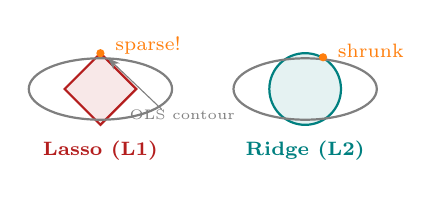
\begin{tikzpicture}[scale=0.65, font=\tiny]
% L1 diamond
\draw[dfred, thick, fill=dfred!10] (1.2,1.0) -- (1.9,1.7) -- (1.2,2.4) -- (0.5,1.7) -- cycle;
\node[dfred, font=\scriptsize\bfseries] at (1.2,0.5) {Lasso (L1)};
% Contour ellipse
\draw[mlgray, thick] (1.2,1.7) ellipse (1.4 and 0.6);
\fill[mlorange] (1.2,2.4) circle (0.08);
\node[mlorange, right, font=\scriptsize] at (1.3,2.55) {sparse!};
% Arrow
\draw[-{Stealth[length=1.5mm]}, mlgray] (2.4,1.3) -- (1.35,2.3);
\node[mlgray, font=\tiny] at (2.8,1.2) {OLS contour};

% L2 circle
\begin{scope}[xshift=4cm]
\draw[dfteal, thick, fill=dfteal!10] (1.2,1.7) circle (0.7);
\node[dfteal, font=\scriptsize\bfseries] at (1.2,0.5) {Ridge (L2)};
% Contour ellipse
\draw[mlgray, thick] (1.2,1.7) ellipse (1.4 and 0.6);
\fill[mlorange] (1.55,2.32) circle (0.08);
\node[mlorange, right, font=\scriptsize] at (1.65,2.45) {shrunk};
\end{scope}
\end{tikzpicture}

\column{0.42\textwidth}
\vspace{2mm}

\includegraphics[width=\textwidth]{06_regularization_comparison/chart.pdf}
\end{columns}

\bottomnote{Use Lasso when you expect many irrelevant features. Use Ridge when all features contribute. Use Elastic Net when unsure.}
\end{frame}

%% FRAME 19: Code Frame
\begin{frame}[fragile]{How Do We Implement This in Python?}
\small
\begin{verbatim}
from sklearn.linear_model import LinearRegression, Ridge, Lasso
from sklearn.model_selection import cross_val_score
from sklearn.preprocessing import StandardScaler

# Prepare data
scaler = StandardScaler()
X_scaled = scaler.fit_transform(X_train)

# OLS
ols = LinearRegression().fit(X_scaled, y_train)
print(f"OLS R2: {ols.score(X_scaled, y_train):.3f}")

# Ridge (L2) with cross-validation
ridge = Ridge(alpha=1.0).fit(X_scaled, y_train)
cv_r2 = cross_val_score(ridge, X_scaled, y_train, cv=5)
print(f"Ridge CV R2: {cv_r2.mean():.3f} +/- {cv_r2.std():.3f}")

# Lasso (L1) -- sparse solution
lasso = Lasso(alpha=0.1).fit(X_scaled, y_train)
n_zero = sum(lasso.coef_ == 0)
print(f"Lasso: {n_zero}/{len(lasso.coef_)} features zeroed out")
\end{verbatim}

\bottomnote{Always scale features before Ridge/Lasso. Use cross-validation (RidgeCV, LassoCV) to tune $\lambda$ automatically.}
\end{frame}

\section{Finance Applications}

%% FRAME 20: CAPM and Factor Models
\begin{frame}[t]{How Does Finance Use Linear Regression Every Day?}
\begin{columns}[T]
\column{0.55\textwidth}
\small
\textbf{Capital Asset Pricing Model (CAPM)}
\[R_i - R_f = \alpha + \beta (R_m - R_f) + \epsilon\]

\begin{compactlist}
\item $\beta$: sensitivity to market risk (systematic)
\item $\alpha$: excess return beyond market exposure
\item $\alpha > 0$ signals manager skill
\end{compactlist}

\vspace{2mm}
\textbf{Fama-French 3-Factor Model}
\[R_i - R_f = \alpha + \beta_1(R_m{-}R_f) + \beta_2 \cdot\text{SMB} + \beta_3 \cdot\text{HML} + \epsilon\]

\begin{compactlist}
\item SMB: Small Minus Big (size premium)
\item HML: High Minus Low (value premium)
\end{compactlist}

\column{0.42\textwidth}
\vspace{2mm}
\footnotesize
\fcolorbox{mlpurple}{mllavender4}{\parbox{0.88\columnwidth}{%
\textbf{Interpretation:}

\vspace{1mm}
$\beta_1 = 1.2$ $\to$ stock moves 1.2\% per 1\% market move

\vspace{1mm}
$\beta_2 = 0.5$ $\to$ tilted toward small caps

\vspace{1mm}
$\beta_3 = -0.3$ $\to$ tilted toward growth

\vspace{1mm}
$\alpha = 0.02$ $\to$ 2\% annual excess return
}}

\vspace{3mm}
\fcolorbox{dfteal}{dfteal!5}{\parbox{0.88\columnwidth}{%
\scriptsize\textbf{Extensions:} Carhart 4-factor (momentum), Fama-French 5-factor (profitability, investment)
}}
\end{columns}

\bottomnote{CAPM (Sharpe, 1964) won the Nobel Prize. Every hedge fund's risk report is built on these regressions.}
\end{frame}

%% FRAME 21: Worked Example -- Factor Model
\begin{frame}[fragile]{Can We Decompose a Fund's Returns Into Risk Factors?}
\small
\textbf{Scenario}: Fund XYZ returned 12\% annually. Is the manager skilled, or just taking risk?

\vspace{2mm}
\begin{verbatim}
import statsmodels.api as sm
# Monthly returns: fund vs factors (60 months)
X = sm.add_constant(factors_df[['Mkt-RF','SMB','HML']])
model = sm.OLS(fund_returns - rf, X).fit()
print(model.summary())
\end{verbatim}

\vspace{1mm}
\footnotesize
\begin{tabular}{lcccc}
\toprule
\textbf{Factor} & \textbf{Coef} & \textbf{Std Err} & \textbf{t-stat} & \textbf{p-value} \\
\midrule
$\alpha$ (intercept) & 0.001 & 0.002 & 0.50 & 0.62 \\
$\beta_{\text{Mkt}}$ (market) & 1.15 & 0.08 & 14.4 & $< 0.001$ \\
$\beta_{\text{SMB}}$ (size) & 0.45 & 0.12 & 3.75 & $< 0.001$ \\
$\beta_{\text{HML}}$ (value) & $-0.20$ & 0.10 & $-2.00$ & 0.05 \\
\bottomrule
\end{tabular}

\vspace{2mm}
\highlight{Verdict}: $\alpha$ is not significant ($p = 0.62$). The 12\% return is explained by high market beta and small-cap tilt -- no evidence of skill.

\bottomnote{Regression-based factor decomposition is the foundation of performance attribution in asset management}
\end{frame}

%% FRAME 22: Decision Flowchart
\begin{frame}[t]{When Should You Use Linear Regression?}
\begin{columns}[T]
\column{0.55\textwidth}
\small
\textbf{Choose linear regression when}:
\begin{compactlist}
\item Target variable is continuous
\item Relationship is approximately linear
\item Interpretability of coefficients matters
\item Fast training is needed
\end{compactlist}

\vspace{3mm}
\textbf{Consider alternatives when}:
\begin{compactlist}
\item Non-linear patterns in residuals $\to$ try polynomial features, trees, or neural nets
\item Binary or categorical target $\to$ logistic regression (L02)
\item Many irrelevant features $\to$ Lasso or tree-based methods
\item Complex interactions $\to$ random forests (L04)
\end{compactlist}

\column{0.42\textwidth}
\vspace{2mm}

\includegraphics[width=\textwidth]{08_decision_flowchart/chart.pdf}
\end{columns}

\bottomnote{Linear regression is always a strong baseline. Start here, check residuals, then decide if you need something more complex.}
\end{frame}

%% ================================================================
%% ZONE 3: CLOSING (frames 23-25)
%% ================================================================

\section{Summary}

%% FRAME 23: Summary
\begin{frame}[t]{Five Key Takeaways}
\small
\begin{enumerate}
\setlength{\itemsep}{6pt}
\item \highlight{The linear model} $\hat{\mathbf{y}} = X\boldsymbol{\beta}$ has a unique closed-form solution $\hat{\boldsymbol{\beta}} = (X^TX)^{-1}X^T\mathbf{y}$ -- derived by minimizing squared residuals
\item \highlight{Model evaluation} requires both metrics ($R^2$, adjusted $R^2$) and visual diagnostics (residual plots, learning curves)
\item \highlight{Gradient descent} is the scalable alternative to OLS -- essential when data is large or the model is extended to non-linear forms
\item \highlight{Regularization} (Ridge, Lasso, Elastic Net) prevents overfitting by trading a small bias increase for a large variance reduction
\item \highlight{Finance applications}: CAPM and factor models are linear regressions -- $\beta$ coefficients decompose risk and return
\end{enumerate}

\bottomnote{Master these five ideas and you have the foundation for all of machine learning}
\end{frame}

%% FRAME 24: References
\begin{frame}[t]{References and Further Reading}
\small
\textbf{Textbooks}
\begin{compactlist}
\item James, Witten, Hastie, Tibshirani (2021). \textit{Introduction to Statistical Learning}, Ch.~3. Free at \texttt{statlearning.com}
\item Hastie, Tibshirani, Friedman (2009). \textit{Elements of Statistical Learning}, Ch.~3. Free at \texttt{hastie.su.domains}
\end{compactlist}

\vspace{3mm}
\textbf{Finance}
\begin{compactlist}
\item Fama, French (1993). Common Risk Factors in the Returns on Stocks and Bonds. \textit{J. Financial Economics}.
\item Sharpe (1964). Capital Asset Prices. \textit{Journal of Finance}.
\end{compactlist}

\vspace{3mm}
\textbf{Practice}
\begin{compactlist}
\item Course notebook: \texttt{L01\_linear\_regression.ipynb} (housing data)
\item sklearn documentation: \texttt{LinearRegression}, \texttt{Ridge}, \texttt{Lasso}
\end{compactlist}

\bottomnote{Start with ISLR Chapter 3 for intuition, then ESL Chapter 3 for the math}
\end{frame}

%% FRAME 25: Closing XKCD
\begin{frame}[t]{The Danger of Extrapolation}
\begin{center}
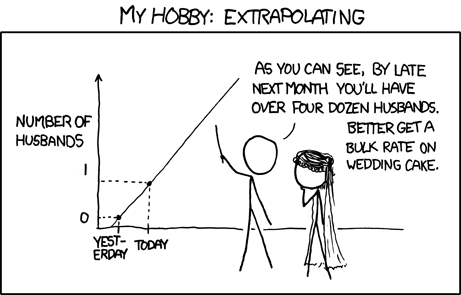
\includegraphics[width=0.55\textwidth]{images/605_extrapolating.png}
\end{center}

\vspace{2mm}
\begin{center}
\small\textit{What happens when you trust your linear model beyond the range of the training data?}
\end{center}

\bottomnote{XKCD \#605 by Randall Munroe (CC BY-NC 2.5)}
\end{frame}

\end{document}
